%%%%%%%%%%%%%%%%%%%%%%%%%%%%%%%%%%%%%%%%%%%%%%%%%%%%%%%%%%%%%%%%%%%%%%%%%%%%%
\chapter{Umsetzung}
\label{chap:Umsetzung}
%%%%%%%%%%%%%%%%%%%%%%%%%%%%%%%%%%%%%%%%%%%%%%%%%%%%%%%%%%%%%%%%%%%%%%%%%%%%%

\section{Technologien}
\subsection{Java}
Die drei Teilprojekte der Arbeit wurden in Java entwickelt. Die verwendete Java Version ist Java 11. Java wird als plattformunabhängige und robuste Programmiersprache verwendet. Auch in der Entwicklung der mobilen Applikation wird Java eingesetzt. Als Alternative zu Java könnte C-Sharp oder eine JavaScript basierende Webserver-Lösung wie Node.js fungieren
\subsection{Android}
Die mobile Applikation ist eine Android-Anwendung. Als Programmiersprache wurde Java verwendet. Eine gute Alternative zu Java bietet Kotlin, da der Code kompakter und einfacher zu schreiben ist ~\parencite{banerjee2018comparative}. Aus Gründen der Einfachheit und Lesbarkeit wurde aber die Programmiersprache Java für die Entwicklung in Android gewählt. Die Applikation wurde sowohl mit einem virtuellen Android-Emulator, als auch mit einem Android-Device getestet.
\subsection{Spring}
Spring, bzw. Spring Boot ist ein Java Framework, das im Zuge der Projektarbeit zur Entwicklungder Web-Applikation verwendet wurde. Spring Boot bietet zusätzlich unter anderem einen eingebetteten Server,  mit dem die Applikation schnell und einfach gestartet werden kann. Auch die Userverwaltung und damit auch die Security-Aspekte wurden mit Spring (Spring Security) entwickelt. Als mögliche Alternative zu Spring mit Spring Security kann Java EE mit einem OAuth2 eingesetzt werden. \ref{pressmarSpring}
\subsection{Maven und Gradle}
Maven ist ein Versionsverwaltungstool mit dem Abhängigkeiten und JARs verwaltetund heruntergeladen werden können. Maven wird hierbei in der Webapplikation und im Plugin eingesetzt. Eine Alternative zu Maven ist das Tool Gradle, welches in der Android Applikation für das Build-Management eingesetzt wurde.
\subsection{Thymeleaf}
Tyhmeleaf ist eine Template-Engine, die in HTML eingesetzt werden kann. Eine Template-Engine nimmt ein vorgefertigtes HTML-Skript (Template) und initialisiert dynamische Werte in die angegebenen Platzhalter. Thymeleaf gehört zu den Server-Side-Engines, das heißt die angezeigte Seite wird am Server generiert ~\parencite{searchmetrics}. Thymeleaf wird in der Webapplikation verwendet, um die Userverwaltung in der Weboberfläche zu implementieren. Der Vorteil dabei ist, da so eine einfache Interaktion mit dem Server stattfinden kann. Diese Interaktion ist beispielsweise die Anmeldung, bei der das angegebene Passwort validiert, überprüft und eine Validierungsnachricht zurückgegeben wird. Als Alternative kann JSF eingesetzt werden. 
\subsection{MongoDB}
Als Datenbank wird die nicht-relationale Lösung MongoDB verwendet, da es verschie-dene Vorteile gegenüber relationales Datenbankmanagementsystem bietet (siehe Punkt4.4.1). Es gehört zu den dokumentorientierten Datenbanken. MongoDB kann über die offiziele Website heruntergeladen und installiert werden. \footnote{https://www.mongodb.com/try/download/community}
\subsection{MongoDB Java Driver}
Der MongoDB Java Driver wird für die Kommunikation (Synchronisation und asyn-chrone Interaktion) mit MongoDB eingesetzt. Mit dem Driver werden unter anderem erstellten Benutzer in die Datenbank gespeichert und ausgelesen.
\subsection{IntelliJ und Android Studio}
Als Entwicklungsumgebungen wurden IntelliJ und Android Studio gewählt, da diese IDEs mehrere verschiedene Sprachen unterstützen und Android Studio eine Abwandlung von IntelliJ ist und daher die Entwicklung sehr einfach und nur minimal unterschiedlich ist.
\subsection{Git und SourceTree}
Git wurde für die Versionsverwaltung verwendet. Ebenso wird in der Applikation mit Git über eine GithubAPI kommuniziert und Daten abgefragt. \footnote{https://developer.github.com/v3/} (siehe Punkt 3.2.1 Konzept: Webapplikation). Statt Git kann auch die Software SVN(Apache Subversion) eingesetzt werden, welches aber verschiedene Nachteile hat wie ein schweres Branch-Handling. Als Git-basiertes Versionsverwaltung-Managementtool wird SourceTree verwendet.

\section{Userverwaltung}
\subsection{Vorteile der Userverwaltung}
Ein Usermanagement mit Sicherheitsimplementierungen ist ein integraler und wichtiger Teil einer Webapplikation, in der sensible Daten behandelt werden, ebenso eignet sich in den gegebenen Anwendungsfällen eine Benutzerverwaltung besonders. Die Userwaltung ergibt daher folgende Vorteile:
\begin{itemize} 
  \item \textbf{Unterstützung für den Benutzer/die Benutzerin} 
Mit der Unterstützung der Userverwaltung können genauere Informationen und Berichte für den angemeldeten Benutzer angezeigt werden. Voraussetzung dafür ist aber die Integration und Verwendung eines Versionsverwaltungs-Management-Tools. So können die Fehler und Probleme der erstellten Files den Entwickler oder der Entwicklerin zugeordnet werden, welcher auf der Weboberfläche eingesehen werden können. So kann der User seine Fehler überblicken und gezielt ausbessern. Durch diese Individualisierung kann auch eine mögliche Verbesserung der Entwicklungsfähigkeit eintreten.  
    \item \textbf{Sicherheit und Zugriffsschutz} \\ Ein anderer wichtiger Punkt ist der Security-Aspekt. Die Webapplikation kann sowohl in einem Unternehmen, oder privat auf einem eigenen Server installiert werden. In beiden Fällen ist ein Zugriffsschutz notwendig, um unberechtigten Benutzer den Zugriff zu verweigern und sensible Daten zu schützen. Die Daten, die in der Webapplikation angezeigt werden müssen sehr vertraulich behandelt werden, da in der Weboberfläche neben weniger wichtigen Code-Smells auch zum Beispiel Sicherheitsprobleme angezeigt werden können. Diese Sicherheitsprobleme können von Angreifern ausgenutzt werden. Auch wenn die Applikation in einem gesicherten Firmennetzwerk installiert wird, ist die Implementierung eines Zugriffsschutzes wichtig. 
\item \textbf{Unterstützung für das Team}
Eigene Entwicklungsteams werden mithilfe einer Benutzerverwaltung erstellt. Dazu können zu den einzelnen Projekten Entwicklerinnen, Entwickler und andere am Projekt beteiligten Personen (Scrum-Master, Tester, usw.) hinzugefügt werden. Nur Mitglieder in diesen Teams können so die Fehler und Bugs einsehen. Den Usern werden daher nur die Projekte angezeigt, an welchen sie auch beteiligt sind. Außerdem können mithilfe der User- und Teamverwaltung eigene und spezielle Reports erstellt werden.
\end{itemize}

\subsection{Allgemeiner Aufbau} 
\subsubsection{User Flow}
Die Benutzerin oder der Benutzer sehen beim Aufrufen der Website, automatisch den Login. Ohne einer richtigen Anmeldung, kann man nicht auf die API oder die Webanwendung zugreifen. Der Benutzerin, der Benutzer muss sich vorher mit einer Email-Adresse und einem Passwort registrieren. Wenn eine Abmeldung nicht manuell erfolgt, so wird der User automatisch abgemeldet.
\subsubsection{Berechtigung zur Datenanzeige}
Um auf Projekt-Inhalte zugreifen zu können, muss ein Projektmitglied die Email-Adresse des neuen Teammitglieds zum Projekt hinzufügen. Erst wenn die Email-Adresse für das Projekt hinterlegt ist, werden die Fehler und Bugs des Projekts angezeigt. Eine andere Möglichkeit dieses Sicherheitsmechanismus wäre eine Anfrage der Entwicklerin oder des Entwicklers an das Team, welches dann die Email-Adresse akzeptieren oder ablehnen kann. So können keine unberechtigten Personen auf sensible Daten zugreifen. Eine Hierarchie-Regelung bzw. verschiedene Berechtigungsstufen sind nicht implementiert, da das Projektteam als Scrum-Team angesehen wird und im Scrum-Prozess alle Mitglieder gleichberechtigt sind \ref{scrumprozess}. Jedes Teammitglied kann daher einen neues Teammitglied mit der Email-Adresse hinzufügen.

\subsection{Implementierung des Usermanagements mit Spring Security}
\subsubsection{Allgemein}
Die Benutzerinnen und Benutzer werden in der Datenbank gespeichert. In der Datenbank wird dazu eine eigene Collection für die User angelegt. Die Passwörter werden verschlüsselt. In der Weboberfläche werden die Daten in einer Thymeleaf-UI eingegeben. Dazu müssen die Dependencies \textit{thymeleaf-layout-dialect} und \textit{spring-boot-starter-security} eingebunden werden. 
\subsubsection{Security Service}   
Im Security Service werden die Userdaten ausgelesen und gespeichert. Das Service implementiert die Spring-Security Schnittstelle \textit{UserDetailsService}. Beim Speichern wird das Passwort des an die Methode übergebenen Users überschrieben (siehe \ref{lst:phase}). Der \textit{BCryptPasswordEncoder} wird hierbei von Spring definiert und verschlüsselt das Passwort als Hash \footnote{https://docs.spring.io/spring-security/site/docs/4.2.15.RELEASE/apidocs/org/springframework/security/crypto/bcrypt/BCryptPasswordEncoder.html}. 

\lstset{
  caption={Speichern und Auslesen des Users.}, 
  basicstyle=\small\ttfamily, 
  label=lst:phase, 
  %float=tbhp, % float image to top/bottom/here/page
  language=Java,
  frame=single,
  breaklines=true, % break long source code lines, and add arrow
  postbreak=\mbox{\textcolor{red}{$\hookrightarrow$}\space},
  %  basewidth={0.55em}, 
  % fontadjust}  % adjust these for more appealing appearance
}

% listing with some settings, such as float, for this listing only
\begin{samepage}% with samepage we keep a FLOATing listing on one page
	\begin{lstlisting}[float=tbhp]
@Autowired
private BCryptPasswordEncoder passwordEncoder;

public void saveUser(User user) {
    user.setPassword(
       passwordEncoder.encode(user.getPassword()));
    mpngoUserService.saveUser(user);
}

@Override
public UserDetails loadUserByUsername(String email) 
  throws UsernameNotFoundException {

    User user = passwordEncoder.findByEmail(email);
    if (user != null) {
      List<GrantedAuthority> authorities =     
        getUserAuthority(user.getRoles());
          return authenticateUser(user, authorities);
    } else {
          throw new UsernameNotFoundException
             ("username not found");
    }
}
	\end{lstlisting}
\end{samepage}
Die Passwort-Überprüfung und der Aufruf der Methode \textit{loadUserByUsername} wird hierbei von Spring selbst implementiert.  Dazu muss das Datenbank-Objekt \textit{User} zum Spring-Objekt \textit{UserDetails} gemappt und eine eigene Configuration-Klassen implementiert werden (siehe Listing \ref{lst:config}). Im Security-Service sind ebenso Berechtigungsüberprüfungen implementiert. Dazu müssen Rollen erstellt und den Benutzer zugewiesen werden. Diese Rollen bzw. Berechtigungen werden mithilfe der \textit{GrantedAuthority} gespeichert und ausgelesen.

\lstset{
  caption={Konfiguration für das Spring Security UserService. Das Service \textit{UserSecurityService} wird nun als das zentrale Service für die Useroperationen von Spring Security verwendet.}, 
  basicstyle=\small\ttfamily, 
  label=lst:config, 
  %float=tbhp, % float image to top/bottom/here/page
  language=Java,
  frame=single,
  breaklines=true, % break long source code lines, and add arrow
  postbreak=\mbox{\textcolor{red}{$\hookrightarrow$}\space},
  %  basewidth={0.55em}, 
  % fontadjust}  % adjust these for more appealing appearance
}

% listing with some settings, such as float, for this listing only
\begin{samepage}% with samepage we keep a FLOATing listing on one page
	\begin{lstlisting}[float=tbhp]
@Bean
public UserDetailsService userDetailService() {
    return new UserSecurityService();
}

@Override
protected void configure
   (AuthenticationManagerBuilder auth) throws Exception {
     UserDetailsService detailsService = userDetailService();
     auth.userDetailsService(detailsService)
        .passwordEncoder(bCryptPasswordEncoder);
}
	\end{lstlisting}
\end{samepage}
Werden hier andere Datenbanken oder Services implementiert, so muss nur die Implementation für das Repository bzw. in diesem Fall das \textit{mpngoUserService} ausgetauscht werden. 
\subsubsection{Security Konfigurationen}
Um die Applikation (URLs der einzelnen Unterseiten) und die API schützen zu können, müssen nun weitere Konfigurationen hinzugefügt werden ~\parencite{springSecBook}. Dazu müssen die einzelnen URLs für die Anzeige der Daten gesichert werden, während hingegen die URLs für den Login und den Website-Aufruf frei zugänglich sein müssen. Auch die Logout-URL kann hier angegeben werden \ref{lst:configurls}.
\lstset{
  caption=[Konfiguration für die Sicherheit der URLs.]{Konfiguration für die Sicherheit der URLs. Die einzelnen Paths können entweder für alle freigegeben oder für eine bestimmte Gruppe angezeigt werden. Das Abmelden wird von Spring automatisch durchgeführt.}, 
  basicstyle=\small\ttfamily, 
  label=lst:configurls, 
  %float=tbhp, % float image to top/bottom/here/page
  language=Java,
  frame=single,
  breaklines=true, % break long source code lines, and add arrow
  postbreak=\mbox{\textcolor{red}{$\hookrightarrow$}\space},
  %  basewidth={0.55em}, 
  % fontadjust}  % adjust these for more appealing appearance
}

% listing with some settings, such as float, for this listing only
\begin{samepage}% with samepage we keep a FLOATing listing on one page
	\begin{lstlisting}[float=tbhp]
...
http.antMatchers("/login").permitAll()
.antMatchers("/reports").hasAuthority("USER")
.and().logout()
.logoutRequestMatcher(new AntPathRequestMatcher("/logout"))
\end{lstlisting}
\end{samepage}
Um auf den Login reagieren zu können, wird ein \textit{AuthenticationSuccessHandler} verwendet, der nach dem Login den User auf die Weboberfläche der Datenanzeige weiterleitet. Hierbei sind im \textit{AuthenticationSuccessHandler} auch noch Überprüfungen implementiert, die den User je nach Rolle (Admin oder User) weiterleiten. 
\subsubsection{Controller und Oberfläche} 
Im Gegensatz zu den anderen Teilen der Webapplikation ist der Login mit Thymeleaf erstellt worden, da so die Login-Überprüfung und das Handling einfach implementiert werden kann. Auch die Navigationsleiste ist mit Thymeleaf implementiert, um auch die Logout-Funktion einfach zu gestalten. Ebenso kann in der Navigationsleiste der angemeldete User eingesehen werden (siehe Abbildung \ref{fig:configuration}). Um Thymeleaf verwenden zu können, ist ein Controller implementiert, der zu den Thymeleaf-Seiten Get-Methoden mit einer \textit{ModelAndView} zur Verfügung stellt. Im \textit{ModelAndView} wird das Model (User) und die View (z.B. Thymeleaf-Login-Page) gespeichert. Als Get-Path wird der Pfad des Thymeleaf-Templates angegeben ~\parencite[Seite 160]{springSecBook}. In der Weboberfläche kann so einfach auf die Daten des Users, zum Beispiel Name und Rechte, zugegriffen werden.
\subsection{Projektkonfiguration für Teammitglieder}
In der Unterseite \textit{Configuration} können die Teammitglieder des Projekts angezeigt und neue Teammitglieder hinzugefügt werden. Dazu muss der angemeldete Benutzer selbst Teil des Teams sein. Um eine neuen User zum Projekt hinzuzufügen muss die Email angegeben werden (siehe Abbildung \ref{fig:configuration}). Der eingeladene User kann daraufhin die Daten des Projekts (Fehler, Bugs, Errors, Charts, usw.) auf der Webseite einsehen. Auf der Konfigurationsseite kann auch eine Projektbeschreibung und ein Link für die Versionsverwaltung hinzugefügt werden (siehe Punkt TODO). Dieser Link dient zur persönlichen Fehler- und Meldungsanzeige sowie zur Verlinkung zum Einsehen der Fehler. (siehe Punkt TODO)
\begin{figure}[tp]
  \centering
  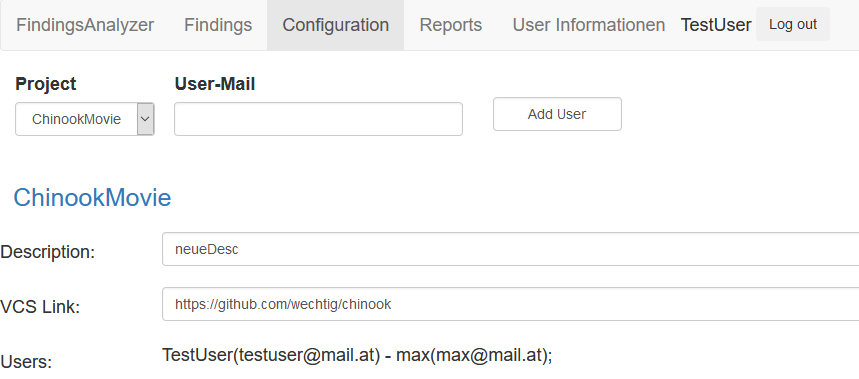
\includegraphics[height=6cm]{images/configuration.PNG}
  % The short caption should be capitalised
  % The full caption should hold a full sentence. 
 \caption[Konfiguration für das Projekt und Team]{Unterseite für verschiedene Konfigurationen für das Projekt und das Team. In diesem Beispiel ist der angemeldete User \textit{TestUser} Mitglied des Teams für das Projekt \textit{ChinookMovie}. So kann er neue Mitglieder zum Team hinzufügen.}
  \label{fig:configuration}
\end{figure}
\section{Anbindung der Versionsverwaltung für spezifische User-Unterstützung}
\subsection{Allgemeines}
Auf der Hauptseite der Webapplikation werden alle Fehler, Code Smells, Warnungen und Bugs gelistet, die die Tools der Statischen Code Analyse im Projekt finden und welche mit den Importer-Plugin in die Datenbank importiert werden. Diese Informationen werden alle in einer Tabelle angezeigt, welche nach Projekt, Klasse oder Datum sortiert und gefiltert werden kann. \\
Das Problem bei dieser Implementierung ist die unspezifische Anzeige: Den Teammitgliedern werden alle Informationen angezeigt, auch Fehler, die von anderen Entwicklerinnen oder Entwicklern implementiert worden sind. So können  Fehler im Projekt gefunden werden und das Team kann die Fehler einsehen. Das Problem bei einer dauerhaften Verbesserung der Kenntnisse der Entwicklerinnen und Entwickler ist hierbei aber die unpersönliche Anzeige. Um den Usern der Webapplikation die genauen Fehler anzuzeigen wird Lösung mit der Anbindung eines VCS-Tools (Version Control System) implementiert. Das Konzept dabei ist es, das die angemeldeten User mit den VCS-Usern verbunden werden. So können die genauen Implementierungen untersucht werden. Dabei werden zum Beispiel die committeden Klassen aus den einzelnen gelesen.
\subsubsection{Ablauf}
Um die spezifische User Unterstützung benutzen zu können, muss im Projekt eine Versionsverwaltung verwendet werden (Im Rahmen dieser Arbeit wurde hierbei die Unterstützung für die Versionsverwaltung Git implementiert). Der Link des Repositories muss zusätzlich in der Projektkonfiguration von einem Teammitglied konfiguriert werden (siehe Abbildung 4.1). Um nun die Accounts der Teammitglieder in der Userverwaltung mit den Entwicklerinnen und Entwicklern des Projekts in der Versionsverwaltung verbinden zu können, wird die Email-Adresse verwendet. Das heißt, die Email-Adresse im Tool der Versionsverwaltung muss mit der Email-Adresse der Userverwaltung übereinstimmen. Werden nun in der Weboberfläche die Informationen zu der Statischen Code Analyse abgefragt, so werden die Informationen in der Datenbank mit den Daten der Versionsverwaltungs-API verglichen und es wird versucht eine Verbindung herzustellen. Es werden nur jene Fehler und Informationen abgefragt und angezeigt, die vom angemeldeten User implementiert und committed worden sind.   
\subsubsection{Alternative Implementierungsmöglichkeiten}
Die beschriebene Methode mit der Einbeziehung eines Versionsverwaltungstools ist nur eine mögliche Methode zur persönlichen Anzeige. Ein Problem bei dieser Methode ist die verpflichtende Angabe eines VCS-Links. Andere Möglichkeiten, die diese Konfiguration nicht verlangen, sind unter anderem: \\
\textbf{Angabe der entwickelnden Klassen und Methoden} \\
Hierbei könnten die Entwicklerinnen und Entwickler die entwickelnden Methoden und Klassen in einer Übersichtsseite auswählen. Fehler, Bugs und andere Meldungen aus diesen Klassen werden den Usern angezeigt.\\
\textbf{Automatische Erkennung durch Verteilung der Aufgaben} \\
Die Idee bei dieser Methode ist eine Konfiguration, wo die Aufgaben verteilt werden: Die Benutzerinnen und Benutzer könnten hierbei jene Packages oder Module angeben, welche sie entwickeln. So können zum Beispiel die Aufgaben als Packages wie Repositories, Modules oder Weboberfläche verteilt werden. \\
\textbf{Autorennamen verwenden} \\
Bei dieser möglichen Lösung werden die Autorangaben der \textit{Javadoc} verwendet. Bei der \textit{Javadoc} zu Klassen werden unter anderem die Autoren angegeben \footnote{https://www.oracle.com/technical-resources/articles/java/javadoc-tool.html}. Dieser Autorenname kann dazu verwendet werden, um den angemeldeten Usern die richtigen Meldungen anzuzeigen, wenn die beiden Namen übereinstimmen.
\subsection{GithubAPI und Service}
\subsection{Oberfläche}
\section{Cron Jobs für regelmäßige Berichte}
\chapterend